\chapter{Amazon EC2}
\section{Description}
Amazon Elastic Compute Cloud (EC2) has been in operation since 2006\ftAmOne, when it commenced its first limited public beta of the service. Since then EC2 has proven extremely popular, and is currently the largest commercially available cloud service with some estimates putting the total number of servers at over 500,000+ servers\ftAmTwo.\ftAmOneText\ftAmTwoText

The EC2 product offering changes nearly monthly, with an enormous variety of products as a part of its offering, including databases (DynamoDB), private clouds (VPC), auto scaling, load balancing (ELB), caching, etc. In the interest of brevity, this report will focus on the core product offering, the ability to create and utilise virtual servers.

The following image displays the login page to the EC2 console, with all the different services that can be administered through the console.

\begin{center}
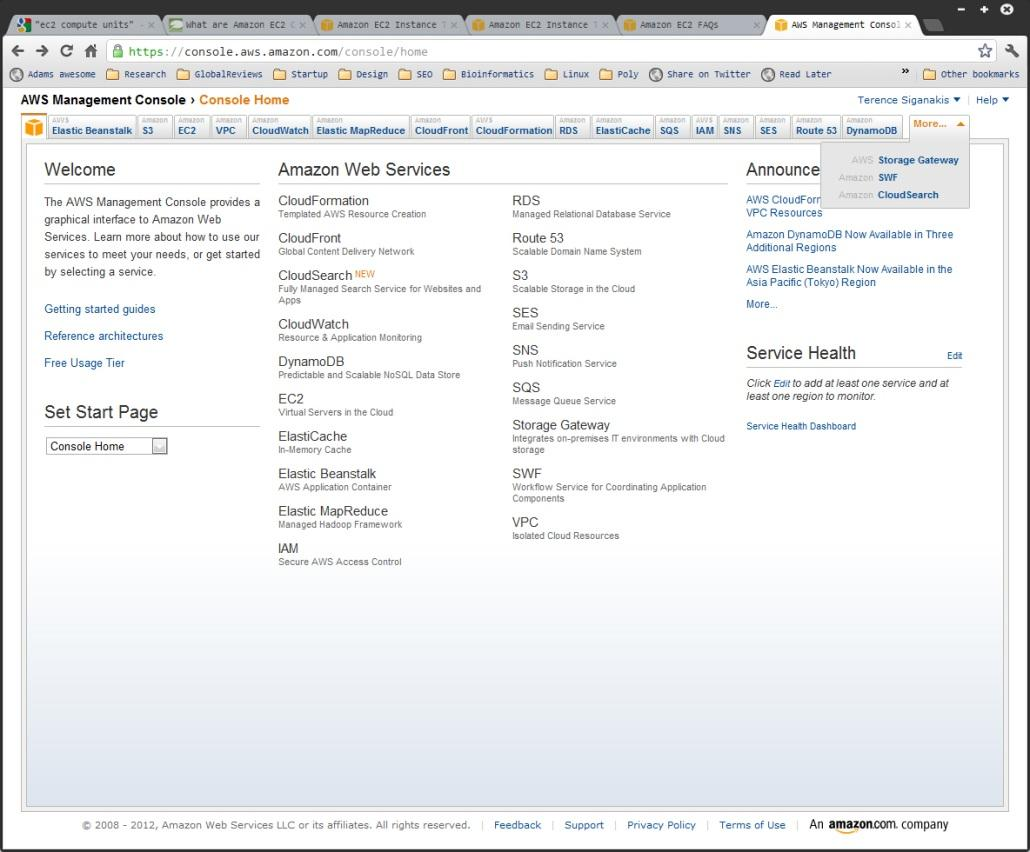
\includegraphics[scale=0.3]{figs/EC2console.jpg}
\end{center}

\section{Instances}
The key abstraction used with Amazon EC2 is that of an ``instance''. An instance is essentially a single computer with a set of specifications. The specifications of instances have their own peculiarities. Each instance type has a set amount of memory, and a set number of ``EC2 Compute Units''. According to the documentation an EC2 Compute unit is described as:
\begin{quote}
The amount of CPU that is allocated to a particular instance is expressed in terms of these EC2 Compute Units. We use several benchmarks and tests to manage the consistency and predictability of the performance of an EC2 Compute Unit. One EC2 Compute Unit provides the equivalent CPU capacity of a 1.0-1.2 GHz 2007 Opteron or 2007 Xeon processor\ftAmThree.\ftAmThreeText
\end{quote}
In the same document, they describe another instance type as having 2 x Xeon X5570 quad core processors which equates to 33.5 compute nodes. So we can assume that a single Xeon X5570 quad core processor is about 16 Compute Units.

EC2 Instances support a variety of different operating systems, including Windows, Linux. In fact it is even possible to create your own instance types by uploading your own VMWare / VirtualBox image. 

Once an instance has been created, it is a fully functional computer to which you have full access (e.g. root in Linux, Administrator in Windows). 

There is no limit to the number of instances that you can spawn, aside from cost. In fact one enterprising company built a 30,000 core cluster (3,809 instances) using EC2 (which can be rented out for \$1,279 per hour)\ftAmFour.\ftAmFourText

\section{Disk Access}
Instances themselves have a small amount of storage associated with them which is essentially utilised for the OS installation. User data is stored using Amazons ``Elastic Block Storage'' (EBS) service, which is a critical aspect of EC2. EBS enables you to create virtual disks of any size and apply them to your instances. These virtual disks can be administered as logical entities separate from the computer that they are connected to. For instance, it is trivial to clone a virtual disk and connect it to a new server. Indeed, this service enables ``Snapshots'', in which all the EBS virtual disks associated with an instance can be duplicated, and a new instance launched from that snapshot.

EC2 Instances and their storage is administered through the EC2 Console, which allows you to launch new instances, clone instances, create virtual disks, assign IP addresses etc. 

More importantly, all these functions can also be completed using the EC2 API, enabling an application to automatically scale itself (add more servers depending on load), or for you to administer your cluster through your iPhone.

\section{Availability \& Reliability}
A key strength of EC2 is the end users ability to specify what data centre instances are launched in. This is done by specifying a region and availability zone. Each availability zone is guaranteed to be in a different datacentre, while each region is geographically separated. At present, EC2 is available in the following regions, US East Coast, US West Coast (Oregon), US West Coast (California), EU West (Ireland), Asia Pacific (Singapore), Asia Pacific (Tokyo), and South America (Sao Paulo). This enables applications to be developed with servers all around the world to reduce latency and improve user experience. It also means that a disaster in one region or with one data centre should not take down your entire cluster.

